\documentclass[10pt]{beamer}
% \documentclass[handout,10pt]{beamer}
\usepackage{my_style}
%%%%%%%%%%%%%%%%%%%%%%%%%%%%%%%%%%%%%%%%%%%%%%%%%%%%%%%%%%%%%%%%%%%%%%%%


\title[Math/CS 375]{Lecture 12 - A}
\subtitle{ \S 5.4 Gaussian Quadrature}

\begin{document}
% -------------------------------------------------
\begin{frame}
  \titlepage
\end{frame}

%%%%%%%%%%%%%%%%%%%%%%%%%%%%%%%%%%%%%%%%%%%
\begin{frame}{Goals}
We will answer these questions:\\[3mm]
\begin{itemize}
    \item What is \textbf{degree of precision}?
    \item In what way are \textbf{Newton-Cotes methods} restrictive?
    \item What is the main idea behind \textbf{Gaussian quadrature}?
    \item How does its \textbf{performance} compare?
\end{itemize}
\end{frame}

%%%%%%%%%%%%%%%%%%%%%%%%%%%%%%%%%%%%%%%%%%%%%%%%%%%%%%%%%%%%%%%%%%%%%%%%
\sectionframe{Degree of Precision}
%%%%%%%%%%%%%%%%%%%%%%%%%%%%%%%%%%%%%%%%%%%%%%%%%%%%%%%%%%%%%%%%%%%%%%%%
\begin{frame}{Degree of Precision}

{
\define{Degree of Precision} % according to Atkinson
{
Suppose an integration method has zero error when applied to a polynomial $p_r(x)$ (assume $r$ is the highest degree). Then we say the method has \textbf{degree of precision} equal to r.
}}

\begin{block}{Note}
    Do not confuse \textbf{order of accuracy} $p$ ($E=\mO(h^p)$) with degree of precision $r$. They are both integers and they are both related to performance of a method. 
\end{block}


\question{
    What is the degree of precision for the Newton-Cotes integration methods?
}



\end{frame}
%%%%%%%%%%%%%%%%%%%%%%%%%%%%%%%%%%%%%%%%%%%%%%%%%%%%%%%%%%%%%%%%%%%%%%%%
\begin{frame}{Degree of Precision}{Trapezoid}

\begin{example}
    \begin{itemize}
        \item Find the exact integral of $y=f(x) = 2x+1 $ on $[1,3]$.
        \item Approximate $\int_1^3 f(x)\, dx$ using the basic trapezoid. 
    \end{itemize}
\end{example}

\begin{itemize}
    \item The exact integral is 

        \begin{align*}
            \int_1^3 2x+1\, dx = \left. x^2 + x\right|_1^3 = 8+2 = 10\\ 
        \end{align*}
    \item The trapezoid approximation is 
        $$
        \int_1^3 2x+1\, dx \approx \frac{f(3)+f(1)}{2}(3-1) = \frac{7+3}{2}(2) = 10
        $$
\end{itemize}

\begin{block}{Note}
    Degree of precision for Trapezoid method is $r=1$.
\end{block}
\end{frame}

\begin{frame}{Visual}

\begin{figure}
    \centering
    \begin{tikzpicture}[scale=1]
    \begin{axis}[
        width=9cm, height=5cm,
        xlabel={$x$}, ylabel={$y$},
        grid=major, 
        thick,
        domain=0:2,
        samples=100,
    ]
        % Define and plot the function f(x) = sin(x)
        \addplot[name path=func, color=blue, thick, domain=1:3] {2*x*+1};
        % \addlegendentry{$f(x) = \sin(x)$};
    
        % Define the x-axis path from x=0 to x=1.5
        \addplot[name path=xaxis, draw=none, domain=1:3] {0};
    
        % Shade the area under f(x) between x=0 and x=1.5
        \addplot [
            fill=blue!20,    % Fill color
            fill opacity=0.3, % Adjust opacity here
            draw=none
        ] fill between [
            of=func and xaxis,
            soft clip={domain=-1:1},
        ];

    \end{axis}
    \end{tikzpicture}\\
\end{figure}
    \begin{itemize}
        \item The integral $\int_1^3 (2x+1)\,dx$ is the area of a trapezoid
        \item This is always true when integrating a linear function
    \end{itemize}
    \keyidea{Trapezoid Method has \textbf{no error} for linear functions.}
\end{frame}
%%%%%%%%%%%%%%%%%%%%%%%%%%%%%%%%%%%%%%%%%%%%%%%%%%%%%%%%%%%%%%%%%%%%%%%%
\begin{frame}{Degree of Precision}{Newton-Cotes}

\begin{itemize}
    \item Recall that Newton-Cotes approximates $f(x)\approx p_n(x)$ and then integrates
        $$I = \int_a^b f(x) \, dx \approx \int_a^b p_n(x)\, dx $$
        
    \item If $f(x) = p_n(x)$, then there cannot be any error 
        $$E = \int_a^b f(x) \, dx - \int_a^b p_n(x)\, dx = \int_a^b f(x)-p_n(x)\,dx = 0$$

    \item Therefore 

    \begin{block}{Note}
        A Newton-Cotes method of degree $n$ has a degree of precision of \underline{at least $n$}, \textit{and sometimes higher}.        
    \end{block}
    
\end{itemize}

\end{frame}

%%%%%%%%%%%%%%%%%%%%%%%%%%%%%%%%%%%%%%%%%%%%%%%%%%%%%%%%%%%%%%%%%%%%%%%
\begin{frame}{Simpson's Rule}
\begin{center}
    
        \begin{tikzpicture}
    \begin{axis}[
        width=9cm, height=4cm,
        xlabel={}, ylabel={},
        grid=major, 
        thick,
        domain=0:2,
        samples=100,
    ]
        % Define and plot the function f(x) = sin(x)
        \addplot[name path=func, color=blue, thick, domain=-1:1] {x^2+1};
        % \addlegendentry{$f(x) = \sin(x)$};
    
        % Define the x-axis path from x=0 to x=1.5
        \addplot[name path=xaxis, draw=none, domain=-1:1] {0};
    
        % Shade the area under f(x) between x=0 and x=1.5
        \addplot [
            fill=blue!20,    % Fill color
            fill opacity=0.3, % Adjust opacity here
            draw=none
        ] fill between [
            of=func and xaxis,
            soft clip={domain=-1:1},
        ];
    \end{axis}
    \end{tikzpicture}\\
\end{center}
\begin{itemize}
    \item  Simpson's rule says 
    $$
        \int_{-1}^1 f(x)\,dx \approx  \frac{1}{3}(f(-1)+4f(0)+f(1))
    $$
    \item If we apply it so $f(x)=x^2+1$ then we get 
    $$
        \int_{-1}^1 f(x)\,dx \approx  \frac{1}{3}(2+4+2)=\frac{8}{3}    $$
    \item This is \textbf{exact}!
\end{itemize}
\end{frame}

%%%%%%%%%%%%%%%%%%%%%%%%%%%%%%%%%%%%%%%%%%%%%%%%%%%%%%%%%%%%%%%%%%%%%%%
\begin{frame}{Degree of Precision for Simpson's}

    \cols{
        \centering
    \begin{tikzpicture}[scale=0.5]
    \begin{axis}[
        width=10cm, height=6cm,
        xlabel={$x$}, ylabel={$y$},
        grid=major, 
        thick,
        domain=0:2,
        samples=100,
    ]
        % Define and plot the function f(x) = sin(x)
        \addplot[name path=func, color=blue, thick, domain=-1:1] {2*x*(x-0.5)*(x+0.25)+3};
        % \addlegendentry{$f(x) = \sin(x)$};
    
        % Define the x-axis path from x=0 to x=1.5
        \addplot[name path=xaxis, draw=none, domain=-1:1] {0};
    
        % Shade the area under f(x) between x=0 and x=1.5
        \addplot [
            fill=blue!20,    % Fill color
            fill opacity=0.3, % Adjust opacity here
            draw=none
        ] fill between [
            of=func and xaxis,
            soft clip={domain=-1:1},
        ];

    \end{axis}
    \end{tikzpicture}\\
    $\int_{-1}^{1} x(x-0.5)(x+0.5)+3\,dx$
    
    }{
    \centering
    \begin{tikzpicture}[scale=0.5]
    \begin{axis}[
        width=10cm, height=6cm,
        xlabel={$x$}, ylabel={$y$},
        grid=major, 
        thick,
        domain=0:2,
        samples=100,
    ]
        % Define and plot the function f(x) = sin(x)
        \addplot[name path=func, color=blue, thick, domain=-1:1] {2*x*(x-0.5)*(x+0.25)+3};
    
        % Define the x-axis path from x=0 to x=1.5
        \addplot[name path=xaxis, draw=none, domain=-1:1] {0};
    
    
        % Plot the linear interpolant (straight line between x=0 and x=1.5)
        \addplot[name path=int, color=black, dashed,thick, domain=-1:1] {-0.5*x^2 + 1.75*x+3};
 
        \addplot [
            fill=blue!20,    % Fill color
            fill opacity=0.3, % Adjust opacity here
            draw=none
        ] fill between [
            of=int and xaxis,
            soft clip={domain=-1:1},
        ];
        % Mark points x=0 and x=1.5 on the curve
        % \addplot[mark=*, only marks, color=red] coordinates {(0, 0) (1.5, 1)};
    \end{axis}
    \end{tikzpicture}
    $\int_{-1}^{1} p_2(x) \,dx$
    }
    \vspace{5mm}
    \begin{itemize}
        \item We know degree of precision is at least 2
        \onslide<2->{
            \item Actually, the degree of precision is 3 - Verify this for Homework! 
            $$\int_{-1}^{1} x(x-0.5)(x+0.5)+3\,dx = \int_{-1}^{1} p_2(x) \,dx$$
        }
    \end{itemize}
\end{frame}
%%%%%%%%%%%%%%%%%%%%%%%%%%%%%%%%%%%%%%%%%%%%%%%%%%%%%%%%%%%%%%%%%%%%%%%%
\begin{frame}{Derivatives in the Error Formulas}

\begin{itemize}
    \item    Trapezoid   $-\frac{(b-a)h^2}{12}f''(\xi)$ 
        $$\text{degree of precision} =1$$
    
    \item Simpson's $1/3$  $-\frac{(b-a)h^4}{90}f^{(4)}(\xi)$ 
        $$\text{degree of precision} =3$$
    \item Simpson's $3/8$  $-\frac{(b-a)h^4}{80}f^{(4)}(\xi)$ 
        $$\text{degree of precision} =3$$
   \item Boole's       $-\frac{2(b-a)h^6}{945}f^{(6)}(\xi)$ 
        $$\text{degree of precision} =5$$
\end{itemize}
    
\end{frame}


%%%%%%%%%%%%%%%%%%%%%%%%%%%%%%%%%%%%%%%%%%%%%%%%%%%%%%%%%%%%%%%%%%%%%%%%
\sectionframe{Gaussian Quadrature}
%%%%%%%%%%%%%%%%%%%%%%%%%%%%%%%%%%%%%%%%%%%%%%%%%%%%%%%%%%%%%%%%%%%%%%%%
\begin{frame}{Quadrature}

\define{Quadrature}{
\begin{itemize}
    \item  \textbf{Numerical Quadratures} are integration rules that can be expressed as the  weighted sum
    $$\int_a^b f(x)\,dx  \approx  \sum_{i=0}^n w_i f(x_i) $$
  \item The $w_i$ are called \textbf{weights}, the $x_i$ are called \textbf{nodes}
\end{itemize}
}
\vspace{5pt}

\begin{itemize}
  \item  Newton-Cotes rules are quadratures with \textbf{equispaced nodes}  
        $$x_i = a+ih, \quad  h=(b-a)/n$$
  \item Example: Simpson's Rule 
$$    \int_0^1 f(x)\,dx \approx \frac{1}{6} f(x_0) + \frac{2}{3}
    f(x_1) + \frac{1}{6}f(x_2)$$
\end{itemize}
\end{frame}
%%%%%%%%%%%%%%%%%%%%%%%%%%%%%%%%%%%%%%%%%%%%%%%%%%%%%%%%%%%%%%%%%%%%%%%%%
\begin{frame}{Newton-Cotes}

\begin{itemize}
    \item Trapezoid       $$\frac{(b-a)}{2}\left[f(a) + f(b)\right]$$
    
   \item Simpson's $1/3$ $$\frac{(b-a)}{6}\left[f(a) + 4f(\frac{a+b}{2}) + f(b)\right]$$
   \item Simpson's $3/8$ $$\frac{(b-a)}{8}\left[f(a) + 3f(a+h) + 3f(b-h) + f(b)\right]$$
   \item Boole's         $$\frac{(b-a)}{90}\left[7f(a) + 32f(a+h) + 12f(\frac{a+b}{2}) + 32f(b-h)+7f(b)\right]$$
\end{itemize}

    \keyidea{Newton-Cotes are a subclass of quadratures with \textbf{equispaced} nodes.}
\end{frame}
%%%%%%%%%%%%%%%%%%%%%%%%%%%%%%%%%%%%%%%%%%%%%%%
\begin{frame}{Degrees of Freedom}{General Quadrature}

{
\define{Degrees of Freedom}{
The number of free parameters in a numerical method is called the \textbf{degrees of freedom}.
}}

\question{
    What is the degrees of freedom for a \emph{general} quadrature with $n+1$ nodes?
}

    $$\sum_{i=0}^n w_i f(x_i) = \underbrace{ \underbrace{w_0}_{free} f(\underbrace{x_0}_{free})  + \cdots + w_n f(x_n)}_{n+1 \;\text{terms}}$$
\begin{itemize} 
    \item $\mathbf{n+1}$ weights 
    \item $\mathbf{n+1}$ node locations
    \item Total: $\mathbf{2n + 2}$
\end{itemize}
\end{frame}
%%%%%%%%%%%%%%%%%%%%%%%%%%%%%%%%%%%%%%%%%%%%%%%%%%%%%%%%%%%%%%%%%%%%%%%%%
\begin{frame}{Degrees of Freedom}{Newton-Cotes}

\question{
    How many free variables are there in a \emph{Newton-Cotes} quadrature with $n+1$ nodes?
}

    $$\sum_{i=0}^n w_i f(x_i) = \underbrace{ \underbrace{w_0}_{free} f(\underbrace{x_0}_{fixed})  + \cdots + w_n f(x_n)}_{n+1 \;\text{terms}}$$
\begin{itemize}
    \item Node locations are \textit{not} free
    \item They must be located at $x_i = a+\frac{b-a}{n}i$
    \item Newton-Cotes has only $\mathbf{n+1}$ free variables

\end{itemize}
\end{frame}
%%%%%%%%%%%%%%%%%%%%%%%%%%%%%%%%%%%%%%%%%%%%%%%%%%%%%%%%%%%%%%%%%%%%%%%%
\begin{frame}{Utilizing Extra Freedom}

\begin{block}{Newton-Cotes vs. General Quadratures}
\begin{itemize}
    \item Newton-Cotes: $n+1$ degrees of freedom 
    \item General quadratures: $2n+2$ degrees of freedom
\end{itemize}
\end{block}

\question{
    If we free up the location of the nodes, 
    what can we with the extra degrees of freedom?
}


\begin{itemize}
  \item We can add extra constraints. 
  \item We can choose to optimize some quantity 
  \item We can optimize a quadrature for \textbf{degree of precision}!
\end{itemize}
\end{frame}

%%%%%%%%%%%%%%%%%%%%%%%%%%%%%%%%%%%%%%%%%%%%%%%%%%%%%%%%%%%%%%%%%%%%%%%%
\begin{frame}{Cubic Function}
    Consider integrating the cubic function over the interval $[1,2]$ $$f(x)=x^3+1$$ 
    \begin{figure}
        \centering
        \begin{tikzpicture}[scale=0.8]
        \begin{axis}[
            width=8cm, height=6cm,
            domain=1:2,
            samples=200,
            axis lines=left,
            ymin=0, ymax=9.5,
            xmin=1, xmax=2,
            xtick={1,1.2,...,2},
            ytick={0,1,...,9},
            xlabel={$x$},
            ylabel={$y$},
            ticklabel style={font=\small},
            title style={yshift=-1ex},
            axis on top,
        ]
        % Fill area under the linear (trapezoid) line
        \addplot [
            name path=base,
            domain=1:2,
            draw=none
        ] {0};
        \addplot [
            name path=trapline,
            domain=1:2,
            draw=none
        ] {7*x - 5};  % line from (1,2) to (2,9)
        \addplot [
            fill=blue!10,
            draw=none
        ] fill between [
            of=trapline and base,
        ];
        % Red curve
        \addplot [
            domain=1:2,
            red,
            thick
        ] {x^3 + 1};
        % Black secant line
        \addplot [
            domain=1:2,
            black,
            thick
        ] {7*x - 5};
        % Endpoints
        \addplot[only marks, mark=o, green, mark size=2pt] coordinates {(1,2) (2,9)};
        % Label the integral value
        \node at (axis cs:1.5,8) {\small $I \approx 5.5000$};
        \end{axis}
        \end{tikzpicture}
    \end{figure}
    \begin{itemize}
        \item The exact answer is 4.75
        \item Trapezoidal rule will yield 5.5 (overshoot)
    \end{itemize}
\end{frame}
%%%%%%%%%%%%%%%%%%%%%%%%%%%%%%%%%%%%%%%%%%%%%%%%%%%%%%%%%%%%%%%%%%%%%%%%
\begin{frame}{Cubic Function}{Moving the Nodes}
  Consider
    \begin{equation*}
      \int_{1}^{2} x^3 + 1\,dx = 4.75
    \end{equation*}
    \begin{columns}
      \begin{column}{0.45\textwidth}
        \begin{tikzpicture}[scale=0.7]
        \begin{axis}[
            width=8cm, height=6cm,
            domain=1:2,
            samples=200,
            axis lines=left,
            ymin=0, ymax=9.5,
            xmin=1, xmax=2,
            xtick={1,1.2,...,2},
            ytick={0,1,...,9},
            xlabel={$x$},
            ylabel={$y$},
            ticklabel style={font=\small},
            title style={yshift=-1ex},
            axis on top,
        ]
        % Fill area under the linear (trapezoid) line
        \addplot [
            name path=base,
            domain=1:2,
            draw=none
        ] {0};
        \addplot [
            name path=trapline,
            domain=1:2,
            draw=none
        ] {7*x - 5};  % line from (1,2) to (2,9)
        \addplot [
            fill=blue!10,
            draw=none
        ] fill between [
            of=trapline and base,
        ];
        % Red curve
        \addplot [
            domain=1:2,
            red,
            thick
        ] {x^3 + 1};
        % Black secant line
        \addplot [
            domain=1:2,
            black,
            thick
        ] {7*x - 5};
        % Endpoints
        \addplot[only marks, mark=*,mark size=2pt,color=green!60!black] coordinates {(1,2) (2,9)};
        % Label the integral value
        \node at (axis cs:1.5,8) {\small $I \approx 5.5000$};
        \end{axis}
        \end{tikzpicture}
      \end{column}
      \begin{column}{0.45\textwidth}
        % \pgfimage[width=5cm]{./figs/quadfig2}
        \begin{tikzpicture}[scale=0.7]
        \begin{axis}[
            width=8cm, height=6cm,
            domain=1:2,
            samples=200,
            axis lines=left,
            ymin=0, ymax=9.5,
            xmin=1, xmax=2,
            xtick={1,1.2,...,2},
            ytick={0,1,...,9},
            xlabel={$x$},
            ylabel={$y$},
            ticklabel style={font=\small},
            title style={yshift=-1ex},
            axis on top,
        ]
        
        % Gauss nodes mapped to [1,2]
        \pgfmathsetmacro{\xA}{(3 + sqrt(3)/3)/2}
        \pgfmathsetmacro{\xB}{(3 - sqrt(3)/3)/2}
        \pgfmathsetmacro{\fA}{(\xA)^3 + 1}
        \pgfmathsetmacro{\fB}{(\xB)^3 + 1}
        
        % Fill under secant line
        \addplot [
            name path=base,
            domain=1:2,
            draw=none
        ] {0};
        
        \addplot [
            name path=secant,
            domain=1:2,
            draw=none
        ] {(\fA - \fB)/(\xA - \xB)*(x - \xB) + \fB};
        
        \addplot [
            fill=blue!10,
            draw=none
        ] fill between[
            of=secant and base,
        ];
        
        % Red curve
        \addplot [
            domain=1:2,
            red,
            thick
        ] {x^3 + 1};
        
        % Black secant line through Gauss points
        \addplot [
            domain=1:2,
            black,
            thick
        ] {(\fA - \fB)/(\xA - \xB)*(x - \xB) + \fB};
        
        % Vertical dashed lines to nodes
        \addplot [dashed, blue, thick] coordinates {(\xA, 0) (\xA, \fA)};
        \addplot [dashed, blue, thick] coordinates {(\xB, 0) (\xB, \fB)};
        
        % Green dots at Gauss nodes
        \addplot[only marks, mark=*, mark size=2pt, color=green!60!black] coordinates {
            (\xA, \fA)
            (\xB, \fB)
        };
        \draw[->](axis cs:1,1) -- (axis cs:1.2,1); 
        \draw[->](axis cs:2,1) -- (axis cs:1.8,1); 

        \node at (axis cs:1.5,8) {\small What's the error?};
        \end{axis}
        \end{tikzpicture}

      \end{column}
    \end{columns}
\question{
    Can we move the nodes $x_0$ and $x_1$ inward so that the error is zero?
}
\end{frame}

%%%%%%%%%%%%%%%%%%%%%%%%%%%%%%%%%%%%%%%%%%%%%%%%%%%%%%%%%%%%%%%%%%%%%%%%
\begin{frame}{Cubic Function}{Moving the Nodes}
  Consider
    \begin{equation*}
      \int_{1}^{2} x^3 + 1\,dx = 4.75
    \end{equation*}
    \begin{columns}
      \begin{column}{0.45\textwidth}
        \begin{tikzpicture}[scale=0.7]
        \begin{axis}[
            width=8cm, height=6cm,
            domain=1:2,
            samples=200,
            axis lines=left,
            ymin=0, ymax=9.5,
            xmin=1, xmax=2,
            xtick={1,1.2,...,2},
            ytick={0,1,...,9},
            xlabel={$x$},
            ylabel={$y$},
            ticklabel style={font=\small},
            title style={yshift=-1ex},
            axis on top,
        ]
        % Fill area under the linear (trapezoid) line
        \addplot [
            name path=base,
            domain=1:2,
            draw=none
        ] {0};
        \addplot [
            name path=trapline,
            domain=1:2,
            draw=none
        ] {7*x - 5};  % line from (1,2) to (2,9)
        \addplot [
            fill=blue!10,
            draw=none
        ] fill between [
            of=trapline and base,
        ];
        % Red curve
        \addplot [
            domain=1:2,
            red,
            thick
        ] {x^3 + 1};
        % Black secant line
        \addplot [
            domain=1:2,
            black,
            thick
        ] {7*x - 5};
        % Endpoints
        \addplot[only marks, mark=*,mark size=2pt,color=green!60!black] coordinates {(1,2) (2,9)};
        % Label the integral value
        \node at (axis cs:1.5,8) {\small $I \approx 5.5000$};
        \end{axis}
        \end{tikzpicture}
      \end{column}
      \begin{column}{0.45\textwidth}
        % \pgfimage[width=5cm]{./figs/quadfig2}
        \begin{tikzpicture}[scale=0.7]
        \begin{axis}[
            width=8cm, height=6cm,
            domain=1:2,
            samples=200,
            axis lines=left,
            ymin=0, ymax=9.5,
            xmin=1, xmax=2,
            xtick={1,1.2,...,2},
            ytick={0,1,...,9},
            xlabel={$x$},
            ylabel={$y$},
            ticklabel style={font=\small},
            title style={yshift=-1ex},
            axis on top,
        ]
        
        % Gauss nodes mapped to [1,2]
        \pgfmathsetmacro{\xA}{(3 + sqrt(3)/3)/2}
        \pgfmathsetmacro{\xB}{(3 - sqrt(3)/3)/2}
        \pgfmathsetmacro{\fA}{(\xA)^3 + 1}
        \pgfmathsetmacro{\fB}{(\xB)^3 + 1}
        
        % Fill under secant line
        \addplot [
            name path=base,
            domain=1:2,
            draw=none
        ] {0};
        
        \addplot [
            name path=secant,
            domain=1:2,
            draw=none
        ] {(\fA - \fB)/(\xA - \xB)*(x - \xB) + \fB};
        
        \addplot [
            fill=blue!10,
            draw=none
        ] fill between[
            of=secant and base,
        ];
        
        % Red curve
        \addplot [
            domain=1:2,
            red,
            thick
        ] {x^3 + 1};
        
        % Black secant line through Gauss points
        \addplot [
            domain=1:2,
            black,
            thick
        ] {(\fA - \fB)/(\xA - \xB)*(x - \xB) + \fB};
        
        % Vertical dashed lines to nodes
        \addplot [dashed, blue, thick] coordinates {(\xA, 0) (\xA, \fA)};
        \addplot [dashed, blue, thick] coordinates {(\xB, 0) (\xB, \fB)};
        
        % Green dots at Gauss nodes
        \addplot[only marks, mark=*, mark size=2pt, color=green!60!black] coordinates {
            (\xA, \fA)
            (\xB, \fB)
        };
        \node at (axis cs:1.5,8) {\small No Error!};

        \draw[->](axis cs:1,1) -- (axis cs:1.2,1); 
        \draw[->](axis cs:2,1) -- (axis cs:1.8,1); 
        \end{axis}
        \end{tikzpicture}

      \end{column}
    \end{columns}

\keyidea{Yes! We can achieve zero error with a trapezoid! }
\end{frame}
%%%%%%%%%%%%%%%%%%%%%%%%%%%%%%%%%%%%%%%%%%%%%%%%%%%%%%%%%%%%%%%%%%%%%%%%%
\begin{frame}{Gaussian Quadrature}
\method{Gaussian Quadrature}
{Integral $\int_a^b f(x)\,dx$, number of points $n+1$}
{Integral approximation}
{The quadrature weights $w_i$ and nodes $x_i$ are chosen to optimize the degree of precision.}

\begin{itemize}
    \item Gaussian Quadrature chooses $w_i$ and $x_i$ so that there is no error for polynomials 
        \begin{align*}
            p_1(x), p_2(x), \cdots, p_k(x)
        \end{align*}
        where $k$ is the highest possible degree
\end{itemize}
\end{frame}

%%%%%%%%%%%%%%%%%%%%%%%%%%%%%%%%%%%%%%%%%%%%%%%%%%%%%%%%%%%%%%%%%%%%%%%%%
\sectionframe{Two-point Gaussian Quadrature}
%%%%%%%%%%%%%%%%%%%%%%%%%%%%%%%%%%%%%%%%%%%%%%%%%%%%%%%%%%%%%%%%%%%%%%%%
\begin{frame}{Domain of Integration}
\begin{itemize}
    \item A general integral $\int_a^b f(x)\,dx$ can be over any interval.

    \item For simplicity, let's stick to the easy integral $[-1, \,1]$. 

    \begin{block}{Odd functions}
        If $f(x)$ is \textbf{odd} ($f(-x)=-f(x)$) then 
        $$ \int_{-1}^{1} f(x) \,dx = 0$$
    \end{block}

    \begin{block}{Even functions}
        If $f(x)$ is \textbf{even} ($f(-x)=f(x)$) then 
        $$ \int_{-1}^{1} f(x) \,dx = 2\int_0^1 f(x)\,dx$$
    \end{block}
\end{itemize}

    
\end{frame}

%%%%%%%%%%%%%%%%%%%%%%%%%%%%%%%%%%%%%%%%%%%%%%%%%%%%%%%%%%%%%%%%%%%%%%%%


\begin{frame}{Gaussian Quadrature with $n=1$}
  \begin{itemize}
    \item Consider the case of $n=1$ (2-points)
    \item Consider $[a,b] = [-1,1]$ for simplicity

    \bigskip
    \begin{block}{Goal}
        Let $p_k(x)$ be an arbitrary polynomial of degree $k$.\\
        Choose $w_0$, $w_1$, $x_0$, $x_1$ so that
            \begin{equation*}
              \int_{-1}^{1} p_k(x)\, dx \approx w_0 p_k(x_0) + w_1 p_k(x_1)
            \end{equation*}
        has \emph{zero error} for $k$ as high as possible.
    \end{block}
  \end{itemize}
\end{frame}
%%%%%%%%%%%%%%%%%%%%%%%%%%%%%%%%%%%%%%%%%%%%%%%%%%%%%%%%%%%%%%%%%%%%%%%%
\begin{frame}{Gaussian Quadrature with $n=1$}{Let's try $p_1(x)$}
\begin{itemize}
    \item In general, $p_1(x) = ax + b$
    \item The exact integral is 
        \begin{equation*}
            \int_{-1}^1 p_1(x) \,dx = (0) a +  (2)b \tag{*} 
        \end{equation*}
    \item The quadrature is 
        \begin{align*}
        \int_{-1}^{1} p_1(x)\, dx &= w_0 p_1(x_0) + w_1 p_1(x_1)\\
                                  &= w_0 (a x_0 + b) + w_1 (a x_1 + b) \\
                                  & = (w_0  x_0 + w_1  x_1)a + (w_0+w_1) b \tag{**}
        \end{align*}
    \item Since we need $(*) = (**)$, we have \textbf{2 conditions} and \textbf{4 unknowns}
    \item Infinite solutions
\end{itemize}
\end{frame}
%%%%%%%%%%%%%%%%%%%%%%%%%%%%%%%%%%%%%%%%%%%%%%%%%%%%%%%%%%%%%%%%%%%%%%%%
\begin{frame}{Gaussian Quadrature with $n=1$}{Let's try $p_2(x)$}
\begin{itemize}
    \item In general, $p_2(x) = ax^2 + bx + c$
    \item The exact integral is 
        \begin{equation*}
        \int_{-1}^1 p_2(x) \,dx = \frac{2}{3} a + 0 b + 2c \tag{*} 
        \end{equation*}
    \item The quadrature is 
        \begin{align*}
        \int_{-1}^{1} p_2(x)\, dx &= w_0 p_k(x_0) + w_1 p_k(x_1)\\
                                  &= w_0 (a x_0^2 + bx_0 + c) + w_1 (a x_1^2 + bx_1 + c) \\
                                  & = (w_0  x_0^2 + w_1  x_1^2)a + (w_0x_0 +w_1x_1) b + (w_0 + w_1)c \tag{**} 
        \end{align*}
    \item  we have \textbf{3 conditions} and \textbf{4 unknowns} $\implies$ infinite solutions
\end{itemize}
\end{frame}
%%%%%%%%%%%%%%%%%%%%%%%%%%%%%%%%%%%%%%%%%%%%%%%%%%%%%%%%%%%%%%%%%%%%%%%%
\begin{frame}{Degree of Precision for $n=1$}

\begin{block}{Goal}
    Find the degree of precision for a simple quadrature of the form
        $$\int_{-1}^1 f(x)\,dx \approx w_0 f(x_0) + w_1 f(x_1) $$
    where the variables $w_0$, $w_1$, $x_0$, and $x_1$ are all free.
\end{block}

\begin{itemize}
\item \textcolor{blue}{\checkmark} Degree $\ge$ 1
\item \textcolor{blue}{\checkmark} Degree $\ge$ 2
\item \textbf{Can we hit 3?}
\end{itemize}
\end{frame}

%%%%%%%%%%%%%%%%%%%%%%%%%%%%%%%%%%%%%%%%%%%%%%%%%%%%%%%%%%%%%%%%%%%%%%%%
\begin{frame}{Derivation}{Part 1}
\begin{block}{Goal}
Find $w_0$, $w_1$, $x_0$, $x_1$ so that the approximation 
$$\int_{-1}^1 f(x) \; \mathit{dx} \approx w_0 f(x_0) + w_1 f(x_1)$$
is exact for any cubic function $f(x) = c_0 + c_1 x + c_2 x^2 + c_3 x^3$.

\end{block}

\begin{itemize}
    \item Exact integral
    \begin{equation*}
        \int_{-1}^1 f(x) \; \mathit{dx} = \int_{-1}^1 \left( c_0 + c_1 x + c_2 x^2 + c_3 x^3 \right) \; \mathit{dx} 
    \end{equation*}
    \item The quadrature
    \begin{equation*}
        w_0 f(x_0) + w_1 f(x_1)= w_0 \left(c_0 + c_1 x_0 + c_2 x_0^2 + c_3 x_0^3 \right) + w_1 \left(c_0 + c_1 x_1 + c_2 x_1^2 + c_3 x_1^3 \right) 
    \end{equation*}
\end{itemize}
\end{frame}
%%%%%%%%%%%%%%%%%%%%%%%%%%%%%%%%%%%%%%%%%%%%%%%%%%%%%%%%%%%%%%%%%%%%%%%%%
\begin{frame}{Derivation}{Part 2}
\begin{itemize}
    \item The exact integral is
    \begin{align*}
    \int_{-1}^1 f(x) \; \mathit{dx} &= \int_{-1}^1 \left( c_0 + c_1 x + c_2 x^2 + c_3 x^3 \right) \; \mathit{dx} \\
                                    &=     2 c_0 + 0 c_1 + \frac{2}{3}c_2 + 0 c_3
    \end{align*}

\item The quadrature is 
    {\small
    \begin{align*}
        w_0 f(x_0) + w_1 f(x_1)&= w_0 \left(c_0 + c_1 x_0 + c_2 x_0^2 + c_3 x_0^3 \right) + w_1 \left(c_0 + c_1 x_1 + c_2 x_1^2 + c_3 x_1^3 \right) \\
        &= c_0(w_0+w_1) + c_1 (w_0x_0 +w_1x_1)  + \cdots \\
         & \hspace{5mm} c_2(w_0x_0^2+w_1x_1^2) + c_3(w_0 x_0^3 + w_1 x_1^3) \\
    \end{align*}
    }
\item We set the quadrature equal to the exact integral 

\item We set the factors of $c_0$, $c_1$, $c_2$, and $c_3$ equal to get 4 equations

\end{itemize}
\end{frame}
%%%%%%%%%%%%%%%%%%%%%%%%%%%%%%%%%%%%%%%%%%%%%%%%%%%%%%%%%%%%%%%%%%%%%%%%
\begin{frame}{Derivation}{Part 3}
\begin{itemize}
    \item Our equations are:
    \begin{eqnarray*}
      w_0 + w_1 = 2 &\qquad&
      w_0x_0 + w_1x_1 =  0 \\
      w_0x_0^2 + w_1x_1^2  = \frac{2}{3} &\qquad&
      w_0x_0^3 + w_1x_1^3 =  0
    \end{eqnarray*}
    \item \textbf{4 equations} and  \textbf{4 unknowns} $\implies$ there is a unique solution
\begin{eqnarray*}
  w_0 = 1 \quad w_1 = 1 \quad x_0 = -\frac{\sqrt{3}}{3}
         \quad x_1 = \frac{\sqrt{3}}{3}
\end{eqnarray*}
\begin{block}{Gaussian Quadrature with $n=1$}
\begin{eqnarray*}
  \int_{-1}^1 f(x) \; \mathit{dx} \approx f\left(-\frac{\sqrt{3}}{3}
  \right) + f\left(\frac{\sqrt{3}}{3} \right)
\end{eqnarray*}
\end{block}
\end{itemize}
\end{frame}

%%%%%%%%%%%%%%%%%%%%%%%%%%%%%%%%%%%%%%%%%%%%%%%%%%%%%%%%%%%%%%%%%%%%%%%%
\begin{frame}{Example 1}
\begin{example}
Approximate $\displaystyle \int_{-1}^{1} x^2 e^{-x} ~dx$ using Gaussian quadrature with $n=1$. \\    
\end{example}
\begin{itemize}
    \item Using the weights $w_0=w_1=1$ and points $x_0 = -\frac{\sqrt{3}}{3}$, $x_1 = \frac{\sqrt{3}}{3}$
    \begin{align*}
    \int_{-1}^1 f(x) \; \mathit{dx} &\approx f\left(-\frac{\sqrt{3}}{3}\right) + f\left(\frac{\sqrt{3}}{3} \right)\\
                                & =\left(-\frac{\sqrt{3}}{3}\right)^2 e^{\frac{\sqrt{3}}{3}} + \left(\frac{\sqrt{3}}{3}\right)^2 e^{-\left(\frac{\sqrt{3}}{3}\right)} \\  
                                & =\frac{1}{3}\left(  e^{\frac{\sqrt{3}}{3}} +e^{-\left(\frac{\sqrt{3}}{3}\right)}\right) \approx 0.7809
    \end{align*}
\end{itemize}
\end{frame}

%%%%%%%%%%%%%%%%%%%%%%%%%%%%%%%%%%%%%%%%%%%%%%%%%%%%%%%%%%%%%%%%%%%%%%%%
\sectionframe{Change of Variables}
%%%%%%%%%%%%%%%%%%%%%%%%%%%%%%%%%%%%%%%%%%%%%%%%%%%%%%%%%%%%%%%%%%%%%%%%
\begin{frame}{Over general interval?}
\begin{alertblock}{Warning!}
The quadrature     
\begin{eqnarray*}
  \int_{-1}^1 f(x) \; \mathit{dx} \approx f\left(-\frac{\sqrt{3}}{3}\right) + f\left(\frac{\sqrt{3}}{3} \right)
\end{eqnarray*}
is only valid when integrating from $-1$ to $1$. 
\end{alertblock}
\begin{itemize}
    \item That means we cannot directly use Gaussian quadrature to approximate integrals over general intervals
    \begin{eqnarray*}
      \int_{a}^b f(x) \; \mathit{dx} 
    \end{eqnarray*}

  \item We can apply a \textbf{change of variables}. Let $ \displaystyle x  = \frac{b-a}{2}t+\frac{b+a}{2}$

\end{itemize}
\end{frame}
%%%%%%%%%%%%%%%%%%%%%%%%%%%%%%%%%%%%%%%%%%%%%%%%%%%%%%%%%%%%%%%%%%%%%%%%

\begin{frame}{Change of Variables in Integration}{General Form}
\begin{block}{General Change of Variables}
    Let $x = g(t)$ be an invertible function. Then 
        $$\int_a^b f(x)\,dx = \int_{g^{-1}(a)}^{g^{-1}(b)} f(g(t)) g'(t)\, dt$$
\end{block}

\begin{itemize}
    \item If we let $$ x = g(t)  = \frac{b-a}{2}t+\frac{b+a}{2}$$  
    \item The inverse is  $t = g^{-1}(x) = \frac{2x - (b+a)}{b-a}$ so 
    \begin{itemize}
        \item $g^{-1}(b) = 1$
        \item $g^{-1}(a) = -1$
    \end{itemize}
    \item The derivative is 
    $$g'(t) = \frac{b-a}{2}$$
    
\end{itemize}
\end{frame}

%%%%%%%%%%%%%%%%%%%%%%%%%%%%%%%%%%%%%%%%%%%%%%%%%%%%%%%%%%%%%%%%%%%%%%%%

\begin{frame}{Remapping the Interval}
\begin{figure}
    \centering
    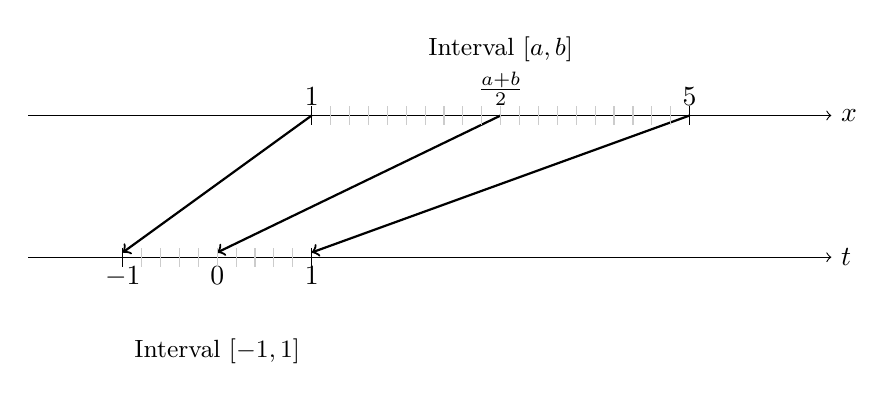
\begin{tikzpicture}[scale=1.2]
    
      % Number lines: x (top), t (bottom)
      \draw[->] (-2,1.5) -- (6.5,1.5) node[right] {$x$};
      \draw[->] (-2,0) -- (6.5,0) node[right] {$t$};
    
      % t-axis ticks: -1, 0, 1
      \foreach \x/\lbl in {-1/{$-1$}, 0/0, 1/1} {
        \draw (\x,0.1) -- (\x,-0.1);
        \node[below] at (\x,0) {\lbl};
      }
    
      % x-axis ticks: a=1, midpoint=3, b=5
      \foreach \x/\lbl in {1/1, 3/{$\frac{a+b}{2}$}, 5/5} {
        \draw (\x,1.6) -- (\x,1.4);
        \node[above] at (\x,1.5) {\lbl};
      }
    
      % Diagonal mapping arrows: from x to t
      \draw[->, thick] (1,1.5) -- (-1,0.05);
      \draw[->, thick] (3,1.5) -- (0,0.05);
      \draw[->, thick] (5,1.5) -- (1,0.05);
    
      % Highlight both intervals with hatching
      \foreach \x in {1.2,1.4,...,4.8} {
        \draw[gray!40] (\x,1.4) -- (\x,1.6); % x interval
      }
      \foreach \x in {-0.8,-0.6,...,0.8} {
        \draw[gray!40] (\x,-0.1) -- (\x,0.1); % t interval
      }
    
      % Optional labels
      \node at (3,2.2) {\small Interval $[a,b]$};
      \node at (0,-1) {\small Interval $[-1,1]$};
    
    \end{tikzpicture}
    \end{figure}
    \begin{block}{Change of Variables}

    The change of variables $$ \displaystyle t = g^{-1}(x) = \frac{2}{b-a}x - \frac{b+a}{b-a}$$
    remaps an interval $x\in[a,b]$ to the interval $t\in[-1,1]$.

    \end{block}
\end{frame}

%%%%%%%%%%%%%%%%%%%%%%%%%%%%%%%%%%%%%%%%%%%%%%%%%%%%%%%%%%%%%%%%%%%%%%%%
\begin{frame}{Change of Variables in Integration}{Applying to Gaussian Quadrature}

\begin{block}{Change of Variables Formula}
Any integral over $[a,b]$ can be changed to an integral over $[-1,1]$ 
\begin{equation*}
    \int_a^b f(x)\,dx = \int_{-1}^{1}
    \underbrace{f\left(\frac{(b-a)t}{2}+\frac{b+a}{2}\right)}_{u(t)}\frac{b-a}{2}\,dt
\end{equation*}
Let us define this function $u(t)$.
\end{block}
  \begin{block}{2-point Gaussian Quadrature for $\int_a^b f(x)\,dx$}
  \begin{equation*}
    \int_a^b f(x)\,dx \approx \frac{b-a}{2} \left[ u\left(-\frac{\sqrt{3}}{3}
  \right) + u\left(\frac{\sqrt{3}}{3}\right)\right], \text{where}
  \end{equation*}
  
  $$u(t) = f\left(\frac{(b-a)t}{2}+\frac{b+a}{2}\right)$$
\end{block}

\end{frame}
%%%%%%%%%%%%%%%%%%%%%%%%%%%%%%%%%%%%%%%%%%%%%%%%%%%%%%%%%%%%%%%%%%%%%%%%%


{ \logo{}
\begin{frame}{Example with Change of Interval}

\begin{example}
Approximate $\displaystyle \int_1^{2} (x^3 +1) ~dx$ using
Gaussian quadrature with $n=1$. \\
\end{example}

   \begin{itemize}
   
      \item Apply the change of variables
        \begin{eqnarray*}
          \int_1^{2} f(x) \; \mathit{dx} = \int_{-1}^1 f\left(\frac{(2-1)t+(2+1)}{2}\right) \;
          \frac{2-1}{2} \; \mathit{dt}
        \end{eqnarray*}

     \item Therefore, we are looking for the integral of
        $$\frac{1}{2}\int_{-1}^1 f\left(\frac{t+3}{2}\right) dt = 
        \frac{1}{2}\int_{-1}^1 \left(\frac{t+3}{2}\right)^3 + 1 ~dt
        $$

     \item Using Gaussian quadrature, our numerical integration becomes:
        $$\frac{1}{2}\left[
            \left(\frac{\sqrt{3}/3+3}{2}\right)^3 + 1
            + \left(\frac{-\sqrt{3}/3+3}{2}\right)^3 + 1
        \right] =
        4.75 \quad (\text{exact!})
        $$

   \end{itemize}
\end{frame}
}

\begin{frame}{Summary}
\begin{itemize}
    \item Standard Trapezoid Rule
    $$
        \int_{-1}^1 f(x) \,dx \approx \frac{h}{2}f(-1) + \frac{h}{2}f(1)
    $$

    \item Gaussian Quadrature 
    $$
          \int_{-1}^1 f(x) \; \mathit{dx} \approx f\left(-\frac{\sqrt{3}}{3}\right) + f\left(\frac{\sqrt{3}}{3} \right)
    $$

    \item Trapezoid is exact for \textbf{linear functions}, but Gauss is exact for \textbf{cubics}!
\end{itemize}
    
\end{frame}
%%%%%%%%%%%%%%%%%%%%%%%%%%%%%%%%%%%%

\begin{frame}{Moving Forward}

\begin{itemize}
    \item General Gaussian Quadrature for $n+1$ points
    \vfill 
    \item Composite Gaussian Quadrature
    \vfill 
    \item Derivation of Nodes and Weights
    \vfill
\end{itemize}
    
\end{frame}

\end{document}
